Das Beispielszenario behandelt eine fiktive Arbeitsvermittlung deren Softwaresystem mit dem  Observer-Pattern umgesetzt wird. In dem Softwaresystem gibt es eine zentrale Komponente JobCenter, welche in regelmäßigen Abständen neue Stellenauschreibungen von externen Arbeitgebern mitgeteilt bekommt. Diese werden auf der Homepage, sowie auf zahllosen Monitoren in der Arbeitsvermittlung aufgelistet. Bei einer neuen Stellenausschreibung soll die Komponente Jobcenter selbständig alle abhängigen Komponenten, wie Homepage und Monitore benachrichtigen, sodass diese sich aktualisieren können.
Für dieses Szenario identifizieren wir das Jobcenter als die Rolle des Subjects und die Homepage und Monitore als Observer. Nachfolgend in Listing \ref{observer_observer_interface} und \ref{observer_subject_interface} sind diese zwei Rollen als Interfaces umgesetzt.
Das Subject definiert neben der Methode \texttt{notifyObsevers()}, zum benachrichtigen aller angemeldeten Observer eine Methode \texttt{attach(Observer)} und \texttt{detach(Observer)} zum An- und Abmelden eines Observers. Das Interface Observer muss hingegen nur zum aktualisieren einer Stellenausschreibung, eine Methode \texttt{update(Offer)} bereitstellen. Der Parameter \texttt{Offer} symbolisiert eine solche Stellenausschreibung, die über die genannte Update-Methode übergeben wird.


\begin{listing}[h!]
   \centering
   \javacode{./resources/observer_Observer_Interface.java}
   \caption{Observer Interface}
    \label{observer_observer_interface}
\end{listing}     
 
\begin{listing}[h!]
   \centering
   \javacode{./resources/observer_Subject_Interface.java}
   \caption{Subject Interface}
    \label{observer_subject_interface}
\end{listing}  
          
  
Im zweiten Schritt wird dann die Klasse Jobcenter (siehe Listing \ref{observer_jobcenter}) implementiert, die von dem Interface Subject erbt und somit die Methoden \texttt{attach(Observer aObserver}, \texttt{detach(Observer aObserver)} und \texttt{notifyObservers()} umsetzt. Zusätzlich initialisiert das Subject eine Collection um die übergebenen Observer über die Attach-Methode zu speichern. Mit der Detach-Methode wird ein Obsever der Collection entfernt. Beim Aufruf der NotifyObserver-Methode wird dieser eine Stellenausschreibung übergeben, die allen gespeicherten Observern über die Update-Methode übergeben wird. 
Nennenswert ist einmal die Tatsache das das Jobangebot an dieser Stelle nur das Interface Observer kennt und das durch die Iteration ausnahmslos alle Observer benachrichtigt werden.

\begin{listing}[h!]
   \centering
   \javacode{./resources/observer_Arbeitsvermittlung.java}
   \caption{Jobcenter}
    \label{observer_jobcenter}
\end{listing} 

Als letztes betrachten wir die Klasse \texttt{Homepage} (siehe Listing \ref{observer_client}). Diese übernimmt die Rolle des Observers indem sie von dem Interface \texttt{Observer} erbt und die Methode \texttt{update(Offer aOffer)} implementiert. 

\begin{listing}[h!]
   \centering
   \javacode{./resources/observer_Klient.java}
   \caption{Observer - Homepage}
    \label{observer_client}
\end{listing}

In Abbildung \ref{observer_sequenz} wird der Ablauf eines solchen Szenarios anhand eines Sequenzdiagramm dargestellt. Zunächst melden sich die Observer \texttt{Homepage} und \texttt{Monitor} am Jobcenter an. Danach wird das JobCenter aktualisiert und alle angemeldeten Observer benachrichtigt.

\begin{figure}[h!]
\centering
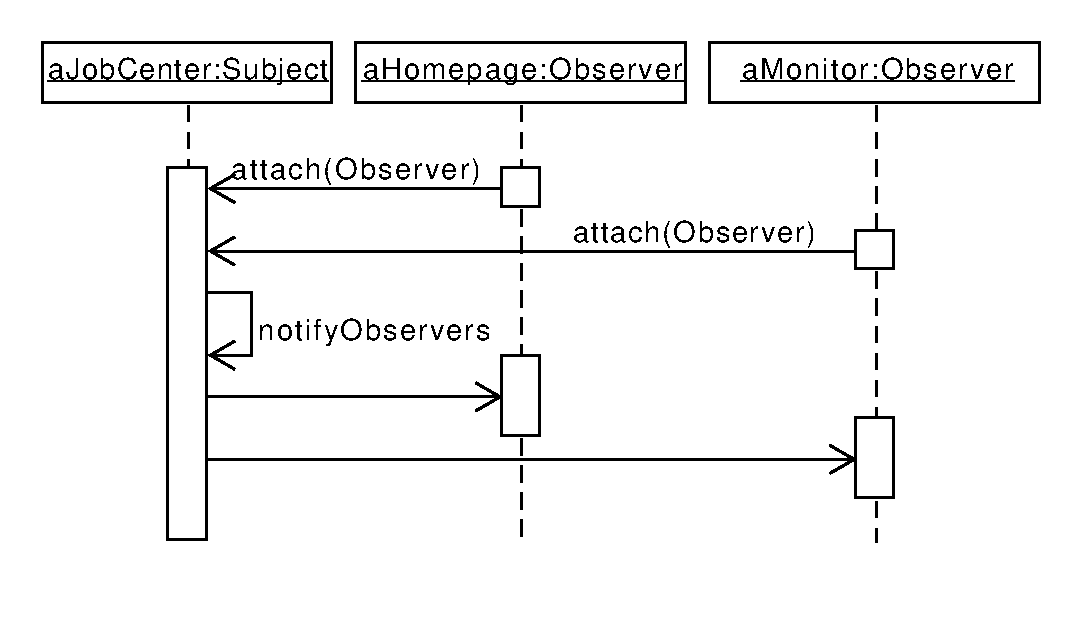
\includegraphics[width=0.7\textwidth]{./paper/observer/observer_sequenz}
\caption{Sequenzdiagramm mit dem Ablauf von JobCenter und desssen Clients}
\label{observer_sequenz}
\end{figure} 